\documentclass[11pt,a4paper]{article}
\usepackage[utf8]{inputenc}
\usepackage[T1]{fontenc}
\usepackage{amsmath,amssymb,amsfonts}
\usepackage{amsthm}
\usepackage[margin=2.5cm]{geometry}
\usepackage{enumitem}
\usepackage{tikz}
\usepackage{xcolor}
\usepackage{hyperref}
\hypersetup{colorlinks=true,linkcolor=blue!55!black,urlcolor=blue!55!black}
\setlist[itemize]{leftmargin=1.4em,itemsep=2pt,topsep=3pt}

% ── theorem environments (all numbered, standard) ──
\newtheorem{theorem}{Theorem}[section]
\newtheorem{lemma}[theorem]{Lemma}
\newtheorem{proposition}[theorem]{Proposition}
\newtheorem{corollary}[theorem]{Corollary}
\theoremstyle{definition}
\newtheorem{definition}[theorem]{Definition}
\newtheorem{example}[theorem]{Example}
\newtheorem{remark}[theorem]{Remark}
\newtheorem{exercise}{Exercise}

% ── macros ──
\newcommand{\Z}{\mathbb{Z}}
\newcommand{\Q}{\mathbb{Q}}
\newcommand{\R}{\mathbb{R}}
\newcommand{\C}{\mathbb{C}}
\newcommand{\F}{\mathbb{F}}
\newcommand{\Spec}{\operatorname{Spec}}
\newcommand{\Frac}{\operatorname{Frac}}
\newcommand{\Hom}{\operatorname{Hom}}
\newcommand{\nil}{\operatorname{nil}}
\newcommand{\rad}{\operatorname{rad}}
\newcommand{\im}{\operatorname{im}}
\newcommand{\p}{\mathfrak{p}}
\newcommand{\q}{\mathfrak{q}}
\newcommand{\m}{\mathfrak{m}}
\newcommand{\fa}{\mathfrak{a}}

\title{
	{\color{blue!40!black}\textbf{\Huge Point}}\\[0.3em]
	\Large \textit{From Number Theory to Algebraic Geometry and Logic}\\[0.7em]
	\large \textbf{Session 1 --- Rings, Ideals, and Spectra}\\[0.3em]
	\normalsize \emph{Complete lecture notes with proofs, examples, and exercises}
}
\author{}
\date{}

\begin{document}
	\maketitle
	\thispagestyle{empty}
	
	\begin{abstract}
		\noindent
		This session builds the first and most concrete incarnation of the course's unifying concept:
		\emph{the prime ideal as a point}. We develop the working language (rings, ideals, quotients,
		localization), prove the characterizations of prime and maximal ideals, establish Krull's
		theorem from Zorn's lemma, and then construct the \emph{spectrum} $\Spec(R)$ with its Zariski
		topology, showing that its points are precisely the prime ideals, its closed points the maximal
		ideals, and that an irreducible space has a \emph{generic point} --- ``the whole space seen as
		one point''. Functoriality of $\Spec$ closes the session and previews the geometric acts.
	\end{abstract}
	
	\subsection*{Session plan (150 minutes)}
	\begin{center}\small
		\begin{tabular}{|l|l|}
			\hline
			\textbf{Time} & \textbf{Block} \\
			\hline
			0:00--0:10 & Orientation: where this session sits in the course; the ``point'' theme \\
			0:10--0:30 & \S1 Rings, ideals, quotients; correspondence theorem \\
			0:30--0:45 & \S2 Localization; primes of $S^{-1}R$; local rings $R_\p$ \\
			0:45--1:10 & \S3 Prime/maximal characterizations; nilradical $=\bigcap$ primes \\
			1:10--1:20 & \emph{Break} \\
			1:20--1:35 & \S4 Zorn's lemma; Krull's theorem \\
			1:35--2:05 & \S5 The spectrum: Zariski topology, $D(f)$, quasi-compactness, generic points \\
			2:05--2:15 & \S6 Functoriality of $\Spec$ \\
			2:15--2:30 & \S7 Gallery of spectra; why Zariski is not Hausdorff; wrap-up \\
			\hline
		\end{tabular}
	\end{center}
	
	\subsection*{Conventions}
	Throughout, \emph{ring} means commutative ring with multiplicative identity $1\neq0$; ring
	homomorphisms send $1$ to $1$; ideals are two-sided (automatic here); $R$ denotes a ring and
	$I,J,\fa$ its ideals. We write $\subseteq$ for inclusion and $\subsetneq$ for proper inclusion.
	
	\tableofcontents
	\newpage
	
	% ══════════════════════════════════════════════
	\section{Rings, Ideals, and Quotients: the Working Language}
	% ══════════════════════════════════════════════
	
	\begin{definition}[Ring]
		A \textbf{ring} is a set $R$ with operations $+$ and $\cdot$ such that $(R,+)$ is an abelian
		group with identity $0$, multiplication is associative and commutative with identity $1\neq0$,
		and multiplication distributes over addition.
	\end{definition}
	
	\begin{example}[Running examples]
		\begin{itemize}
			\item $\Z$, $\Q$, $\R$, $\C$; finite fields $\F_p=\Z/p\Z$.
			\item Polynomial rings $k[x]$, $k[x,y]$; $\Z[x]$.
			\item Quadratic integer rings $\Z[i]$, $\Z[\sqrt{-5}]$.
			\item Quotient rings $\Z/n\Z$, $k[x]/(f)$ (defined below).
		\end{itemize}
		These examples will carry every definition of the course; test each new notion on all of them.
	\end{example}
	
	\begin{definition}[Ideal; generated; principal]
		An \textbf{ideal} $I\subseteq R$ is an additive subgroup with $rI\subseteq I$ for all $r\in R$.
		For $S\subseteq R$, the \textbf{ideal generated by $S$} is
		$(S)=\{\sum_{\text{finite}} r_i s_i : r_i\in R,\ s_i\in S\}$, the smallest ideal containing $S$.
		An ideal is \textbf{principal} if $I=(a)$ for one element; \textbf{proper} if $I\neq R$.
	\end{definition}
	
	\begin{definition}[Quotient ring]
		For an ideal $I$, the \textbf{quotient ring} $R/I$ is the set of cosets $r+I$ with
		$(r+I)+(s+I)=(r+s)+I$ and $(r+I)(s+I)=rs+I$; the projection $\pi:R\to R/I$, $r\mapsto r+I$, is a
		surjective homomorphism with kernel $I$.
	\end{definition}
	
	\begin{proposition}[Universal property of the quotient]
		If $\varphi:R\to S$ is a homomorphism with $I\subseteq\ker\varphi$, there is a unique homomorphism
		$\bar\varphi:R/I\to S$ with $\bar\varphi\circ\pi=\varphi$.
	\end{proposition}
	
	\begin{theorem}[Correspondence theorem]\label{thm:correspondence}
		Let $I\subseteq R$ be an ideal. The maps
		\[
		J\longmapsto \pi^{-1}(J)\quad\text{and}\quad \fa\longmapsto \pi(\fa)=\fa/I
		\]
		give an inclusion-preserving bijection between ideals of $R/I$ and ideals of $R$ containing $I$.
		Under this bijection, prime ideals correspond to prime ideals and maximal to maximal.
	\end{theorem}
	\begin{proof}
		Standard verifications show $\pi^{-1}(J)$ is an ideal of $R$ containing $I$, and $\pi(\fa)$ an ideal
		of $R/I$; the two maps are inverse since $\pi$ is surjective. For primality: if $\bar x\bar y\in\fa/I$
		with lifts $x,y$, then $xy\in\fa$, so $x\in\fa$ or $y\in\fa$, hence $\bar x\in\fa/I$ or $\bar y\in\fa/I$.
		Maximality follows because $(R/I)/(\fa/I)\cong R/\fa$ (third isomorphism), and a ring is a field
		exactly when its only ideals are $0$ and itself (Theorem~\ref{thm:prime-max} below).
	\end{proof}
	
	\begin{example}
		\begin{itemize}
			\item Ideals of $\Z/n\Z$ correspond to divisors $d\mid n$; e.g.\ ideals of $\Z/12\Z$ are
			$(\bar1),(\bar2),(\bar3),(\bar4),(\bar6),(\bar0)$; the maximal ones are $(\bar2),(\bar3)$.
			\item $k[x]/(f)$: if $f$ is irreducible this is a field (a finite extension of $k$); if
			$f=\prod f_i^{e_i}$ the ring has nilpotents and several maximal ideals $(\bar f_i)$.
			\item $\C[x,y]/(y-x^2)\cong\C[t]$: the coordinate ring of a parabola.
		\end{itemize}
	\end{example}
	
	% ══════════════════════════════════════════════
	\section{Localization}
	% ══════════════════════════════════════════════
	
	\begin{definition}[Multiplicatively closed set; localization]
		A subset $S\subseteq R$ is \textbf{multiplicatively closed} if $1\in S$ and $s,t\in S\Rightarrow st\in S$.
		The \textbf{localization} $S^{-1}R$ is the set of fractions $r/s$ modulo
		$\frac{r}{s}=\frac{r'}{s'}\iff \exists\,t\in S:\ t(rs'-r's)=0$, with the usual fraction operations;
		$\iota:R\to S^{-1}R$, $r\mapsto r/1$, is a homomorphism with $\ker\iota=\{r:\exists s\in S,\ sr=0\}$.
	\end{definition}
	
	\begin{example}
		\begin{itemize}
			\item $S=R\setminus\{0\}$, $R$ a domain: $S^{-1}R=\Frac(R)$; e.g.\ $\Frac(\Z)=\Q$, $\Frac(k[x])=k(x)$.
			\item $S=R\setminus\p$ for a prime $\p$: write $R_\p$; e.g.\ $\Z_{(p)}=\{a/b:p\nmid b\}$.
			\item $S=\{1,f,f^2,\dots\}$: write $R_f$; e.g.\ $k[x]_x=k[x,x^{-1}]$.
		\end{itemize}
	\end{example}
	
	\begin{proposition}[Universal property of localization]
		If $\varphi:R\to T$ sends every $s\in S$ to a unit of $T$, there is a unique $\tilde\varphi:S^{-1}R\to T$
		with $\tilde\varphi\circ\iota=\varphi$.
	\end{proposition}
	
	\begin{proposition}[Primes of a localization]\label{prop:loc-primes}
		The maps $\q\mapsto\iota^{-1}(\q)$ and $\p\mapsto\p S^{-1}R$ give an inclusion-preserving bijection
		\[
		\Spec(S^{-1}R)\ \longleftrightarrow\ \{\p\in\Spec R:\ \p\cap S=\varnothing\}.
		\]
	\end{proposition}
	\begin{proof}
		If $\q\in\Spec(S^{-1}R)$ then $\p:=\iota^{-1}(\q)$ is prime and $\p\cap S=\varnothing$ (elements of $S$
		map to units, and a unit cannot lie in a proper ideal). Conversely, for $\p$ with $\p\cap S=\varnothing$,
		the set $\p S^{-1}R=\{p/s:p\in\p,s\in S\}$ is an ideal; it is proper since $1\notin\p S^{-1}R$
		(otherwise $t\cdot1\in\p$ for some $t\in S$). It is prime: if $(r/s)(r'/s')=rr''/ss'\in\p S^{-1}R$ then
		$t rr'\in\p$ for some $t\in S$, so $rr'\in\p$ (as $t\notin\p$), hence $r\in\p$ or $r'\in\p$. The two maps
		are mutually inverse by direct computation.
	\end{proof}
	
	\begin{corollary}\label{cor:local}
		For a prime $\p$, the ring $R_\p$ is \textbf{local}: its only maximal ideal is $\p R_\p$, and
		$R_\p/\p R_\p\cong\Frac(R/\p)=:\kappa(\p)$, the \textbf{residue field} at $\p$.
	\end{corollary}
	\begin{proof}
		By Proposition~\ref{prop:loc-primes}, ideals of $R_\p$ correspond to ideals of $R$ contained in $\p$;
		hence $\p R_\p$ is the unique maximal ideal. The residue field identification follows from
		$R_\p/\p R_\p\cong (R/\p)_{\bar0\text{-complement}}=\Frac(R/\p)$.
	\end{proof}
	
	% ══════════════════════════════════════════════
	\section{Prime and Maximal Ideals}
	% ══════════════════════════════════════════════
	
	\begin{definition}[Prime ideal]
		A proper ideal $\p\subsetneq R$ is \textbf{prime} if $ab\in\p\Rightarrow a\in\p$ or $b\in\p$.
	\end{definition}
	\begin{definition}[Maximal ideal]
		A proper ideal $\m\subsetneq R$ is \textbf{maximal} if there is no ideal with $\m\subsetneq I\subsetneq R$.
	\end{definition}
	
	\begin{theorem}[Characterizations]\label{thm:prime-max}
		For a proper ideal $I\subsetneq R$:
		\begin{enumerate}[label=(\alph*)]
			\item $I$ is prime $\iff R/I$ is an integral domain.
			\item $I$ is maximal $\iff R/I$ is a field.
		\end{enumerate}
	\end{theorem}
	\begin{proof}
		(a) $R/I$ a domain means $\bar a\bar b=0\Rightarrow\bar a=0$ or $\bar b=0$, i.e.\
		$ab\in I\Rightarrow a\in I$ or $b\in I$.
		
		(b) If $R/I$ is a field and $I\subseteq J\subseteq R$, pick $x\in J\setminus I$ if $J\neq I$; then
		$\bar x\neq0$ is invertible, so $1=\bar x\bar y=\overline{xy}$, hence $1\in J$, so $J=R$.
		Conversely if $I$ is maximal and $\bar x\neq0$, then $I+(x)=R$, so $1=i+rx$ for some $i\in I$,
		whence $\bar1=\bar r\bar x$ and $\bar x$ is invertible; thus $R/I$ is a field.
	\end{proof}
	
	\begin{corollary}
		Every maximal ideal is prime.
	\end{corollary}
	\begin{proof}
		A field is an integral domain; apply Theorem~\ref{thm:prime-max}.
	\end{proof}
	
	\begin{example}
		In $\Z$: $(p)$ is maximal (and prime) for primes $p$; $(0)$ is prime but \emph{not} maximal.
		In $k[x,y]$: $(x)$ is prime (quotient $k[y]$, a domain) but not maximal; $(x,y)$ is maximal
		(quotient $k$); $(x^2)$ is neither (quotient has nilpotents).
	\end{example}
	
	\begin{definition}[Nilradical]
		The \textbf{nilradical} $\nil(R)=\{x\in R:x^n=0 \text{ for some } n\ge1\}$.
	\end{definition}
	
	\begin{proposition}\label{prop:nilradical}
		$\nil(R)$ is an ideal, and $\nil(R)=\bigcap_{\p\in\Spec R}\p$.
	\end{proposition}
	\begin{proof}
		If $x^n=0,y^m=0$ then $(x+y)^{n+m}=0$ by the binomial theorem (each term has $x^i$ with $i\ge n$ or
		$y^j$ with $j\ge m$), and $(rx)^n=0$; so $\nil(R)$ is an ideal. Every prime contains all nilpotents
		($x^n\in\p\Rightarrow x\in\p$), giving $\nil(R)\subseteq\bigcap\p$.
		
		For the reverse, suppose $x\notin\nil(R)$; then $S=\{1,x,x^2,\dots\}$ is multiplicatively closed with
		$0\notin S$. Let $\Sigma$ be the set of ideals disjoint from $S$, ordered by inclusion; $\Sigma\neq\varnothing$
		($(0)\in\Sigma$). Zorn's lemma (Section~\ref{sec:zorn}) gives a maximal element $\p\in\Sigma$. We claim
		$\p$ is prime: if $a,b\notin\p$ then $\p+(a)$ and $\p+(b)$ meet $S$, so $x^i=p_1+ra$, $x^j=p_2+sb$;
		multiplying, $x^{i+j}\in\p+(ab)$, so $\p+(ab)$ meets $S$, forcing $ab\notin\p$. Hence $\p\in\Spec R$,
		$x\notin\p$, so $x\notin\bigcap\p$.
	\end{proof}
	
	\begin{definition}[Jacobson radical]
		The \textbf{Jacobson radical} $J(R)=\bigcap_{\m\text{ maximal}}\m$. Always $\nil(R)\subseteq J(R)$.
	\end{definition}
	\begin{remark}
		$\nil(R)$ measures ``functions vanishing to infinite order everywhere''; $J(R)$ measures elements
		invertible-modulo-every-point. For $\Z$ both are $0$; for $\Z/p^n\Z$ both equal $(\bar p)$.
	\end{remark}
	
	% ══════════════════════════════════════════════
	\section{Zorn's Lemma and the Existence of Maximal Ideals}\label{sec:zorn}
	% ══════════════════════════════════════════════
	
	\begin{theorem}[Zorn's lemma (axiom)]
		If every chain in a nonempty partially ordered set $(\Sigma,\le)$ has an upper bound in $\Sigma$,
		then $\Sigma$ has a maximal element.
	\end{theorem}
	
	\begin{theorem}[Krull]\label{thm:krull}
		Every proper ideal of a ring $R$ is contained in a maximal ideal. In particular every nonzero ring
		has at least one maximal ideal, and $\Spec R\neq\varnothing$.
	\end{theorem}
	\begin{proof}
		Let $I\subsetneq R$ and let $\Sigma$ be the set of proper ideals containing $I$, ordered by inclusion;
		$\Sigma\neq\varnothing$. If $\{I_\alpha\}$ is a chain, set $J=\bigcup_\alpha I_\alpha$: $J$ is an ideal
		(unions of chains of ideals are ideals) and $J\neq R$ (else $1\in I_\alpha$ for some $\alpha$). So $J\in\Sigma$
		is an upper bound; Zorn gives a maximal element $\m\in\Sigma$, which is a maximal ideal containing $I$.
		Since $(0)$ is proper, a maximal ideal exists; and maximal ideals are prime, so $\Spec R\neq\varnothing$.
	\end{proof}
	
	\begin{remark}[Where the axiom reappears]
		The same argument (or its relatives) returns in Session~3 (existence of algebraic closures) and
		Session~58 (Deligne's theorem: coherent topoi have enough points). Flag it for students: these are
		the three places the course genuinely uses choice.
	\end{remark}
	
	% ══════════════════════════════════════════════
	\section{The Spectrum of a Ring}
	% ══════════════════════════════════════════════
	
	\begin{definition}[Spectrum]
		The \textbf{spectrum} of $R$ is the set $\Spec R=\{\p\subseteq R:\p\text{ prime}\}$.
	\end{definition}
	
	\begin{definition}[Closed sets $V(I)$]
		For an ideal $I$, set $V(I)=\{\p\in\Spec R:I\subseteq\p\}$. Declare the sets $V(I)$ to be the
		\textbf{closed sets} of the \textbf{Zariski topology} on $\Spec R$.
	\end{definition}
	
	\begin{proposition}[Zariski axioms]\label{prop:zariski}
		\begin{enumerate}[label=(\alph*)]
			\item $V(0)=\Spec R$ and $V(R)=\varnothing$.
			\item $V\!\big(\sum_\alpha I_\alpha\big)=\bigcap_\alpha V(I_\alpha)$.
			\item $V(I\cap J)=V(IJ)=V(I)\cup V(J)$.
		\end{enumerate}
		Hence the $V(I)$ are exactly the closed sets of a topology.
	\end{proposition}
	\begin{proof}
		(a) Every prime contains $0$; no proper prime contains $1$.
		(b) $\p\supseteq\sum_\alpha I_\alpha \iff \p\supseteq I_\alpha$ for all $\alpha$.
		(c) $IJ\subseteq I\cap J\subseteq I$ gives $V(I)\subseteq V(I\cap J)\subseteq V(IJ)$; for the reverse,
		if $\p\supseteq IJ$ but $\p\nsupseteq I$ and $\p\nsupseteq J$, pick $a\in I\setminus\p$, $b\in J\setminus\p$;
		then $ab\in IJ\subseteq\p$ with $a,b\notin\p$, contradicting primality. So $V(IJ)=V(I)\cup V(J)$,
		and the displayed inclusions force $V(I\cap J)=V(IJ)$ as well.
	\end{proof}
	
	\begin{lemma}\label{lem:V-radical}
		$V(I)=V(\rad I)$, where $\rad I=\{x:x^n\in I\}$; moreover $\rad I=\bigcap_{\p\supseteq I}\p$.
	\end{lemma}
	\begin{proof}
		Apply Proposition~\ref{prop:nilradical} in $R/I$: $\nil(R/I)=\rad I/I=\bigcap_{\p\supseteq I}\p/I$.
		Since $V(I)$ depends only on the set of primes containing $I$, and $\rad I$ has the same containing
		primes as $I$, the equality $V(I)=V(\rad I)$ follows.
	\end{proof}
	
	\begin{definition}[Basic opens]
		For $f\in R$, $D(f)=\Spec R\setminus V((f))=\{\p:f\notin\p\}$.
	\end{definition}
	
	\begin{proposition}[The $D(f)$ form a basis]\label{prop:Df-basis}
		\begin{enumerate}[label=(\alph*)]
			\item $D(f)\cap D(g)=D(fg)$.
			\item $\bigcup_i D(f_i)=\Spec R \iff (f_i: i)=R$.
			\item The $D(f)$ form a basis of the Zariski topology.
		\end{enumerate}
	\end{proposition}
	\begin{proof}
		(a) $f\notin\p$ and $g\notin\p$ $\iff$ $fg\notin\p$ (primality).
		(b) $\bigcup_i D(f_i)=\Spec R$ means no prime contains all $f_i$, i.e.\ $V((f_i))=\varnothing$; by
		Lemma~\ref{lem:V-radical} this means $\rad((f_i))=\bigcap_{\p}\p$ over primes containing $(f_i)$ is all of $R$,
		i.e.\ $(f_i)=R$ (else Krull gives a maximal, hence prime, ideal containing it).
		(c) Every open is $\Spec R\setminus V(I)=\bigcup_{f\in I}D(f)$, and (a) gives stability under finite
		intersection; hence the $D(f)$ form a basis.
	\end{proof}
	
	\begin{theorem}[Quasi-compactness of $\Spec$]\label{thm:qc}
		$\Spec R$ is quasi-compact: every open cover has a finite subcover. In fact each $D(f)$ is quasi-compact.
	\end{theorem}
	\begin{proof}
		Let $D(f)\subseteq\bigcup_i D(g_i)$. Then $V((f))\supseteq\bigcap_i V((g_i))=V((g_i:i))$, so by
		Lemma~\ref{lem:V-radical}, $f^n\in(g_i:i)$ for some $n$: $f^n=\sum_{j=1}^N r_j g_{i_j}$. Any prime
		containing all $g_{i_j}$ contains $f^n$, hence $f$; contrapositively $D(f)\subseteq\bigcup_{j=1}^N D(g_{i_j})$.
		Taking $f=1$ gives quasi-compactness of $\Spec R$.
	\end{proof}
	
	\begin{lemma}[Closure of a point]\label{lem:closure}
		For $\p\in\Spec R$, the closure of $\{\p\}$ is $V(\p)=\{\q:\q\supseteq\p\}$.
	\end{lemma}
	\begin{proof}
		$\overline{\{\p\}}$ is the smallest closed set containing $\p$, i.e.\ the intersection of all $V(I)$
		with $\p\in V(I)$, i.e.\ all $V(I)$ with $I\subseteq\p$; the smallest such closed set is $V(\p)$ since
		$I\subseteq\p\Rightarrow V(\p)\subseteq V(I)$.
	\end{proof}
	
	\begin{corollary}[Closed points]
		$\p$ is a closed point of $\Spec R$ $\iff$ $\p$ is a maximal ideal.
	\end{corollary}
	\begin{proof}
		$\{\p\}$ closed $\iff V(\p)=\{\p\}$ $\iff$ no prime strictly contains $\p$ $\iff$ $\p$ maximal.
	\end{proof}
	
	\begin{definition}[Generic point]
		A point $\eta\in\Spec R$ is \textbf{generic} if $\overline{\{\eta\}}=\Spec R$.
	\end{definition}
	\begin{example}
		If $R$ is an integral domain then $(0)$ is the unique generic point: $\overline{\{(0)\}}=V(0)=\Spec R$.
		In $\Spec\Z$ the generic point is $(0)$; every nonempty open contains it. More generally the generic
		points of $\Spec R$ are the minimal primes.
	\end{example}
	
	\begin{definition}[Specialization]
		We say $\p$ \textbf{specializes} to $\q$ (write $\p\rightsquigarrow\q$) if $\q\in\overline{\{\p\}}$,
		i.e.\ $\p\subseteq\q$. Closed points are ``the most special''; generic points ``the most general''.
	\end{definition}
	
	\begin{figure}[h]
		\centering
		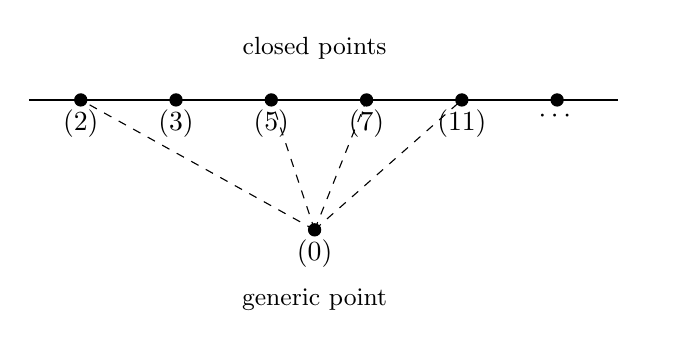
\begin{tikzpicture}[scale=1.1]
			\draw[thick] (-0.6,0) -- (6.2,0);
			\foreach \x/\l in {0/(2),1.1/(3),2.2/(5),3.3/(7),4.4/(11),5.5/\cdots}{
				\filldraw (\x,0) circle (2pt) node[below] {$\l$};
			}
			\node at (6.6,0) {};
			\filldraw (2.7,-1.5) circle (2pt) node[below] {$(0)$};
			\draw[dashed] (2.7,-1.5) -- (0,0);
			\draw[dashed] (2.7,-1.5) -- (2.2,0);
			\draw[dashed] (2.7,-1.5) -- (3.3,0);
			\draw[dashed] (2.7,-1.5) -- (4.4,0);
			\node at (2.7,-2.3) {\small generic point};
			\node at (2.7,0.6) {\small closed points};
		\end{tikzpicture}
		\caption{$\Spec\Z$: one closed point per prime, plus the generic point $(0)$ whose closure is everything.}
	\end{figure}
	
	% ══════════════════════════════════════════════
	\section{Functoriality of the Spectrum}
	% ══════════════════════════════════════════════
	
	\begin{proposition}\label{prop:functorial}
		Let $\varphi:R\to S$ be a ring homomorphism. For $\q\in\Spec S$, the preimage $\varphi^{-1}(\q)$ is a
		prime ideal of $R$; the assignment
		\[
		\varphi^*:\Spec S\longrightarrow\Spec R,\qquad \q\longmapsto\varphi^{-1}(\q)
		\]
		is continuous. Moreover $(\psi\circ\varphi)^*=\varphi^*\circ\psi^*$ and $(\mathrm{id})^*=\mathrm{id}$,
		so $\Spec$ is a contravariant functor $\mathbf{Ring}\to\mathbf{Top}$.
	\end{proposition}
	\begin{proof}
		Primality: if $ab\in\varphi^{-1}(\q)$ then $\varphi(a)\varphi(b)=\varphi(ab)\in\q$, so
		$\varphi(a)\in\q$ or $\varphi(b)\in\q$. Continuity: for an ideal $I\subseteq R$,
		$(\varphi^*)^{-1}(V(I))=\{\q:\ I\subseteq\varphi^{-1}(\q)\}=\{\q:\ \varphi(I)\subseteq\q\}
		=V(\varphi(I)S)$, a closed set. Functoriality is direct computation.
	\end{proof}
	
	\begin{example}
		\begin{itemize}
			\item $\Z\hookrightarrow\Q$: $\Spec\Q=\{(0)\}\to\Spec\Z$ lands on the generic point $(0)$.
			\item $\Z\twoheadrightarrow\Z/n\Z$: $\Spec(\Z/n\Z)\to\Spec\Z$ lands on the primes dividing $n$.
			\item $k\hookrightarrow k[x]$: the closed point $(x-a)$ maps to $(0)$ --- ``a point of the line
			lies over the generic point of the ground field''; this is the first hint that fibres matter (S30).
		\end{itemize}
	\end{example}
	
	\begin{remark}[Why contravariant, and why it matters]
		Points \emph{pull back}: a map of rings $R\to S$ lets an $S$-point be viewed as an $R$-point. This is
		exactly the functor-of-points philosophy made rigorous in Session~29 ($X\cong\Hom(-,X)$) and again in
		Session~54 (a topos point is a morphism $\mathbf{Set}\to\mathcal E$). The theme ``point $=$ morphism
		into the object'' starts here.
	\end{remark}
	
	% ══════════════════════════════════════════════
	\section{A Gallery of Spectra; the Zariski Topology is Strange}
	% ══════════════════════════════════════════════
	
	\begin{example}[Gallery]
		\begin{itemize}
			\item $\Spec\Z$: closed points $(p)$, one generic $(0)$ (figure above).
			\item $\Spec\C[x]$: closed points $(x-a)$, $a\in\C$, plus generic $(0)$ --- the affine line.
			\item $\Spec\R[x]$: closed points $(x-a)$ and $(x^2+bx+c)$ with $b^2-4c<0$ (conjugate pairs), plus $(0)$.
			\item $\Spec\C[x,y]$: closed points $(x-a,y-b)$; curve-generic points $(f)$ for irreducible $f$;
			the generic $(0)$. A two-dimensional space with three layers of points.
			\item $\Spec\Z_{(p)}$: exactly two points, $(pR_{(p)})$ closed and $(0)$ generic (Corollary~\ref{cor:local}).
			\item $\Spec\C[x,y]/(xy)$: two crossing lines; the crossing point $(x,y)$ is where the space fails
			to be a manifold --- a first taste of singularities (S25, S30).
		\end{itemize}
	\end{example}
	
	\begin{remark}[Not Hausdorff, but $T_0$]
		In $\Spec\Z$, any two nonempty opens meet: $D(m)\cap D(n)=D(mn)\neq\varnothing$ since $(mn)\neq\Z$ has
		a prime over it. So the Zariski topology is never Hausdorff for infinite spectra. It is however $T_0$:
		distinct points have distinct closures (Lemma~\ref{lem:closure}). This ``coarseness'' is a feature:
		the topology remembers \emph{algebraic} specialization, not metric proximity. Compare with the
		$p$-adic and analytic topologies of Sessions~17--19 and 37--38, and with the \'etale topology of
		Session~52, which repairs exactly this deficiency.
	\end{remark}
	
	% ══════════════════════════════════════════════
	\section{Exercises}
	% ══════════════════════════════════════════════
	\begin{exercise}
		List all ideals of $\Z/36\Z$; identify the prime and the maximal ones; draw the inclusion poset.
	\end{exercise}
	\begin{exercise}
		Prove that $k[x,y]/(y-x^2)\cong k[t]$. What happens for $k[x,y]/(y^2-x^3)$? (Is it a domain? Is it
		isomorphic to $k[t]$?)
	\end{exercise}
	\begin{exercise}
		Show $\nil(\Z/n\Z)$ equals the ideal generated by the product of the distinct primes dividing $n$.
		Compute $\nil(\Z/72\Z)$.
	\end{exercise}
	\begin{exercise}
		Prove that a ring $R$ is a field $\iff$ its only ideals are $0$ and $R$ $\iff$ every nonzero element
		is a unit. Deduce that a homomorphism from a field is injective or zero.
	\end{exercise}
	\begin{exercise}
		Describe $\Spec\R[x]$ completely (closed points, generic point) and compare with $\Spec\C[x]$.
		Which points of $\Spec\C[x]$ lie over a given point of $\Spec\R[x]$ under the map of
		Proposition~\ref{prop:functorial}?
	\end{exercise}
	\begin{exercise}
		Prove that $D(f)=\varnothing\iff f\in\nil(R)$, and that $D(f)=\Spec R\iff f$ is a unit.
	\end{exercise}
	\begin{exercise}
		Show $\Spec R$ is irreducible (not a union of two proper closed subsets) $\iff$ $\nil(R)$ is a prime
		ideal $\iff$ $\Spec R$ has a generic point.
	\end{exercise}
	\begin{exercise}
		Let $\varphi:\Z\to\Z[i]$ be the inclusion. Describe the fibres of $\varphi^*:\Spec\Z[i]\to\Spec\Z$
		over $(2)$, $(3)$, $(5)$, and $(0)$. (This is decomposition of primes in a quadratic extension ---
		the concrete preview of Sessions~9 and~20.)
	\end{exercise}
	\begin{exercise}
		Prove that the localization functor $S^{-1}(-)$ is exact: it sends short exact sequences of
		$R$-modules to short exact sequences. (Uses Session~2 language; do after Session~2 if preferred.)
	\end{exercise}
	\begin{exercise}
		Give an example of a ring whose Jacobson radical is strictly larger than its nilradical, and one
		where they coincide but are nonzero.
	\end{exercise}
	
	% ══════════════════════════════════════════════
	\section*{Where This Session Feeds the Course}
	\addcontentsline{toc}{section}{Where This Session Feeds the Course}
	% ══════════════════════════════════════════════
	\begin{itemize}
		\item \textbf{Depends on:} nothing (first session); P1--P3 supply group/topological language as needed.
		\item \textbf{Feeds:} S2 (modules over $R$, fibres $M\otimes_R\kappa(\p)$); S24 (Dedekind domains,
		prime factorization); S28 (schemes $=$ glued spectra with structure sheaf); S30 (morphisms, fibres);
		S46 (decomposition/inertia over primes); S52--S54 (Zariski site, topos points); Zorn reused in S3, S58.
		\item \textbf{Unifying thread:} the prime ideal is the first incarnation of ``point''; the generic
		point is ``the whole space seen as one point''; specialization is the arrow from general to special;
		$\Spec$ functoriality is the first appearance of ``point $=$ morphism into the object''.
	\end{itemize}
	
	\subsection*{References for this session}
	\begin{enumerate}[label={[\arabic*]}]
		\item Atiyah, M.F. \& Macdonald, I.G. \emph{Introduction to Commutative Algebra}, ch.1--3.
		\item Eisenbud, D. \emph{Commutative Algebra with a View Toward Algebraic Geometry}, ch.2, 4.
		\item Vakil, R. \emph{The Rising Sea}, ch.3--4.
		\item Hartshorne, R. \emph{Algebraic Geometry}, ch.II \S2 (for the scheme-theoretic sequel).
		\item Matsumura, H. \emph{Commutative Ring Theory}, ch.1--2 (supplementary).
	\end{enumerate}
	
	\vspace{1.5em}
	\begin{center}
		\rule{0.6\textwidth}{0.4pt}\\[0.5em]
		\textit{End of Session 1 --- next: Session 2, Modules, Tensor Products, and Exact Sequences}
	\end{center}
	
\end{document}